\section{Diagramas de clases}

\noindent
En el desarrollo de un sistema software, una de las partes fundamentales, para obtener buenos resultados, es analizar y diseñar el sistema, y esto no solo se refiere a interfaces de usuario, sino a la estructura del sistema, las clases que lo componen y la forma en que éstas interactúan entre sí para que todo funcione de forma adecuada.
\newline
Para ESCOMobile se consideran los siguientes diagramas de clases:
\newline
\newline
\noindent
Primeramente, mostramos el diagrama de clases general, en donde se pueden observar todas las clases del sistema y la forma en que se relacionan, posteriormente se muestran pequeños fragmentos que representan una porción del diagrama general, para comprender la estructura de una mejor forma.

\pagebreak
\begin{figure}[!htpb]
	\hypertarget{fig:clasesGeneral}{\hspace{1pt}}
	\begin{center}
		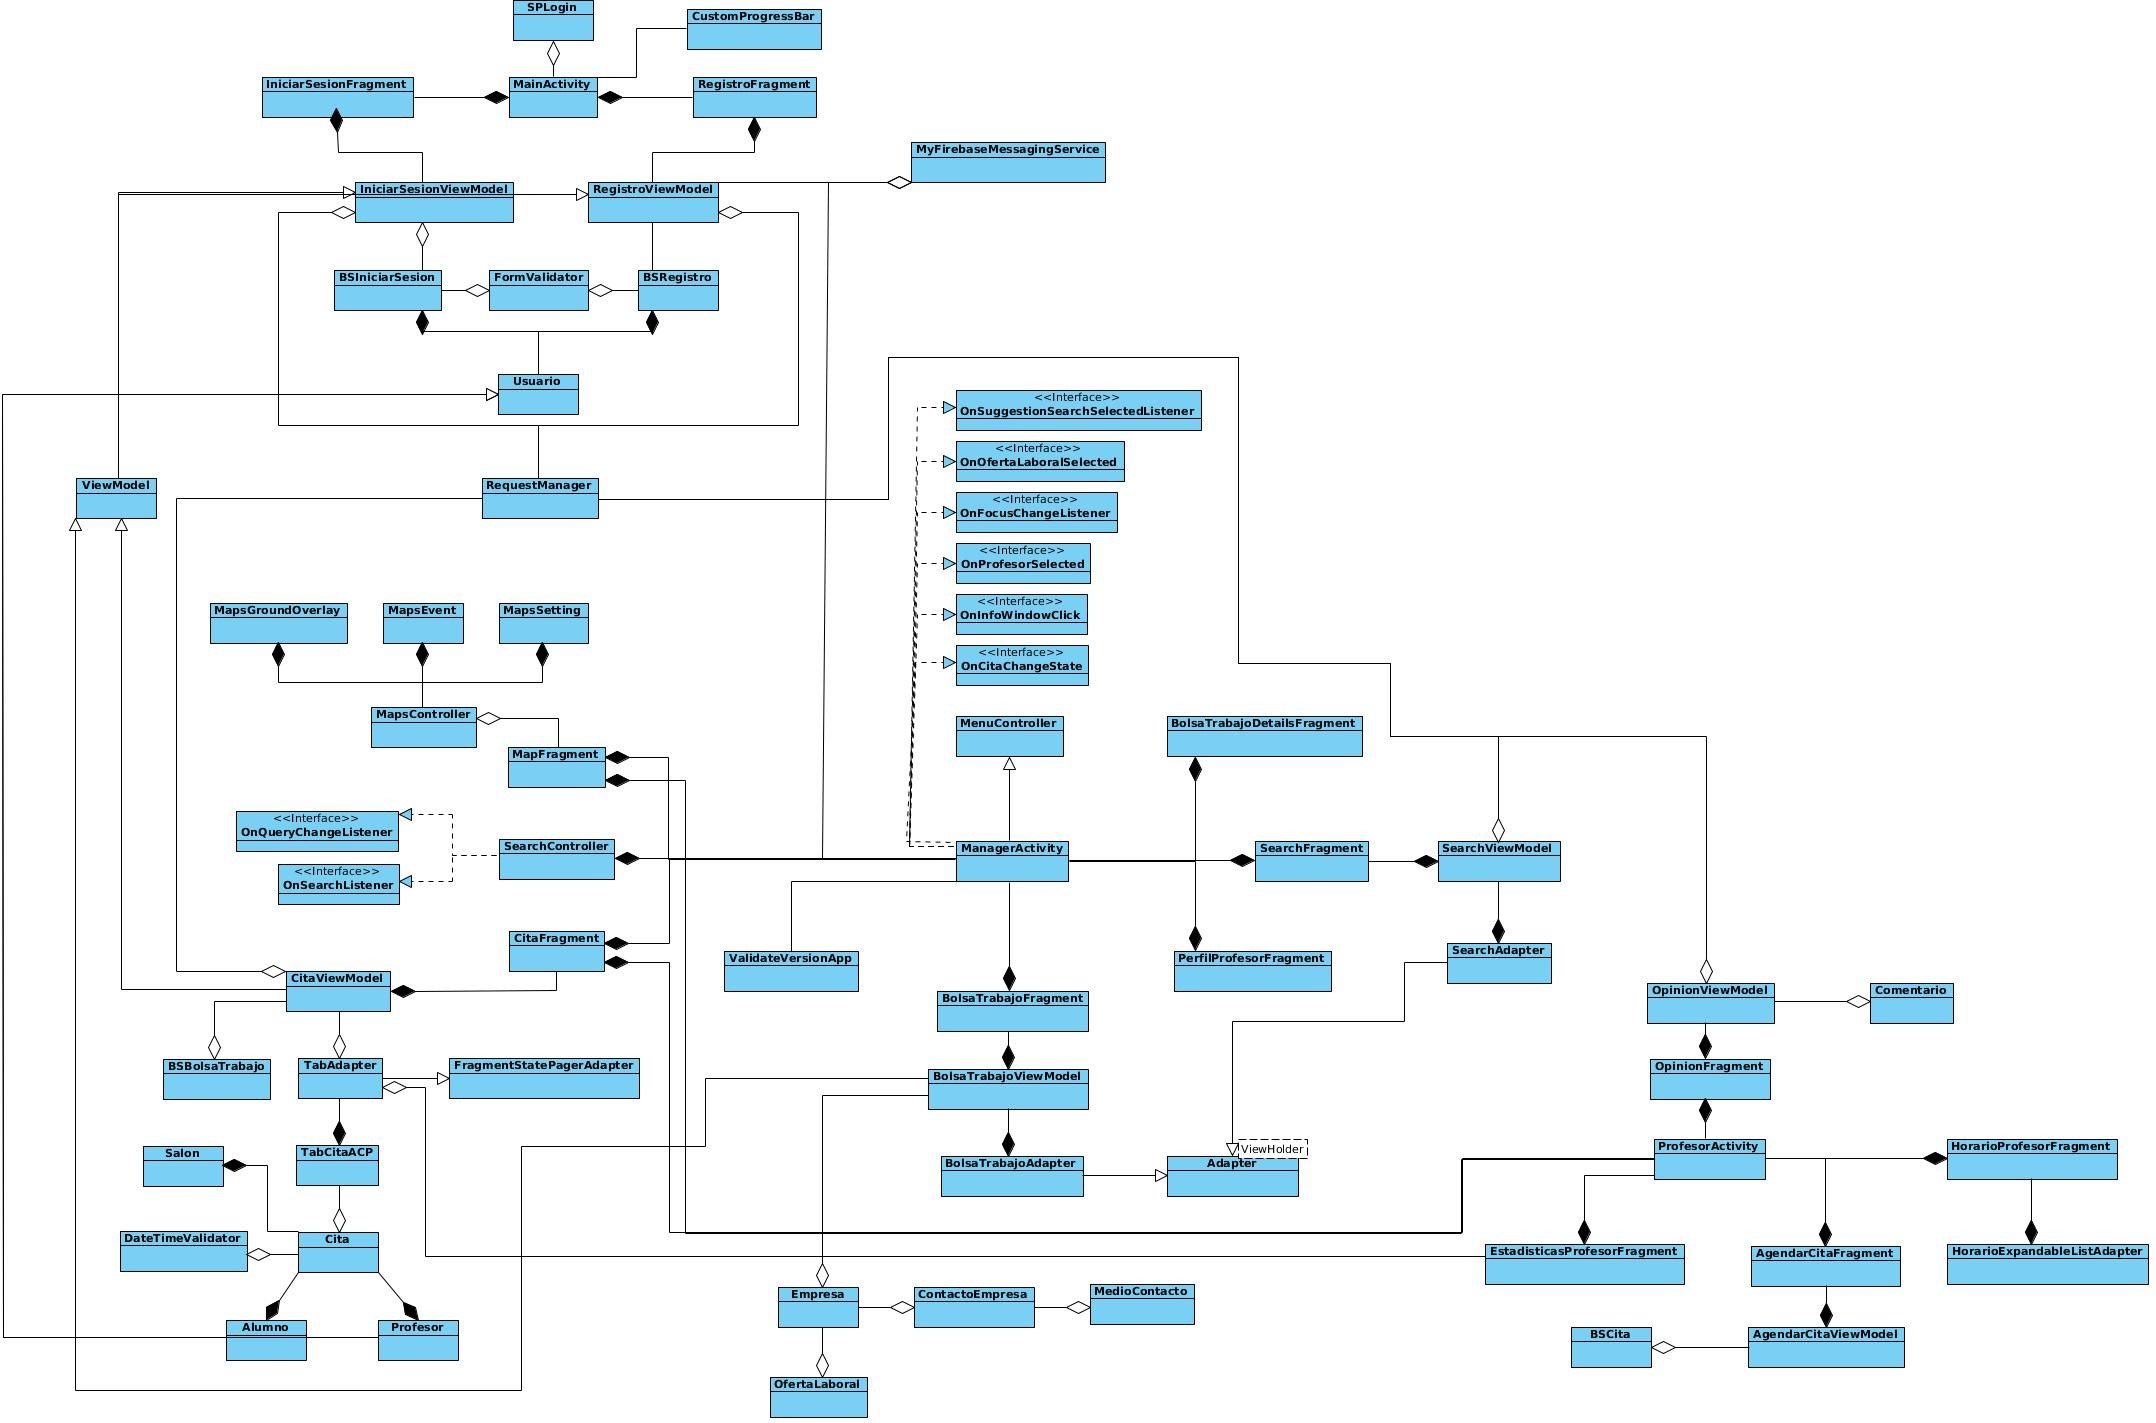
\includegraphics[width=1\textwidth]{images/clases/DiagramaClasesGeneralESCOMobileApp}
		\caption{Diagrama de clases general de ESCOMobile.}
		\label{fig:clasesGeneral}
	\end{center}
\end{figure}

\begin{figure}[!htpb]
	\hypertarget{fig:clasesContBusqueda}{\hspace{1pt}}
	\begin{center}
		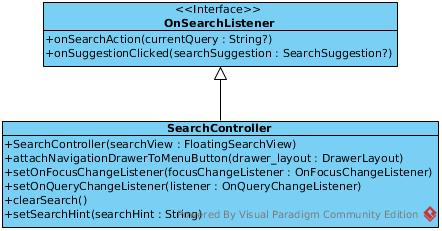
\includegraphics[width=1\textwidth]{images/clases/ControladorBusqueda}
		\caption{Diagrama de clases: Controlador Búsqueda.}
		\label{fig:clasesContBusqueda}
	\end{center}
\end{figure}

\begin{figure}[!htpb]
	\hypertarget{fig:clasesContMap}{\hspace{1pt}}
	\begin{center}
		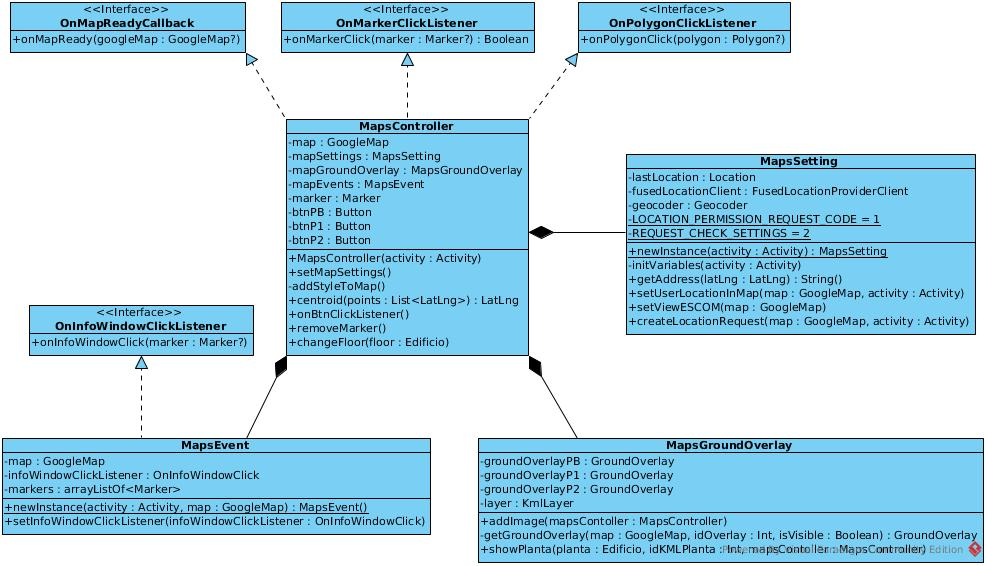
\includegraphics[width=1\textwidth]{images/clases/ControladorMapa}
		\caption{Diagrama de clases: Controlador Mapa.}
		\label{fig:clasesContMap}
	\end{center}
\end{figure}

\begin{figure}[!htpb]
	\hypertarget{fig:clasesModEntidad}{\hspace{1pt}}
	\begin{center}
		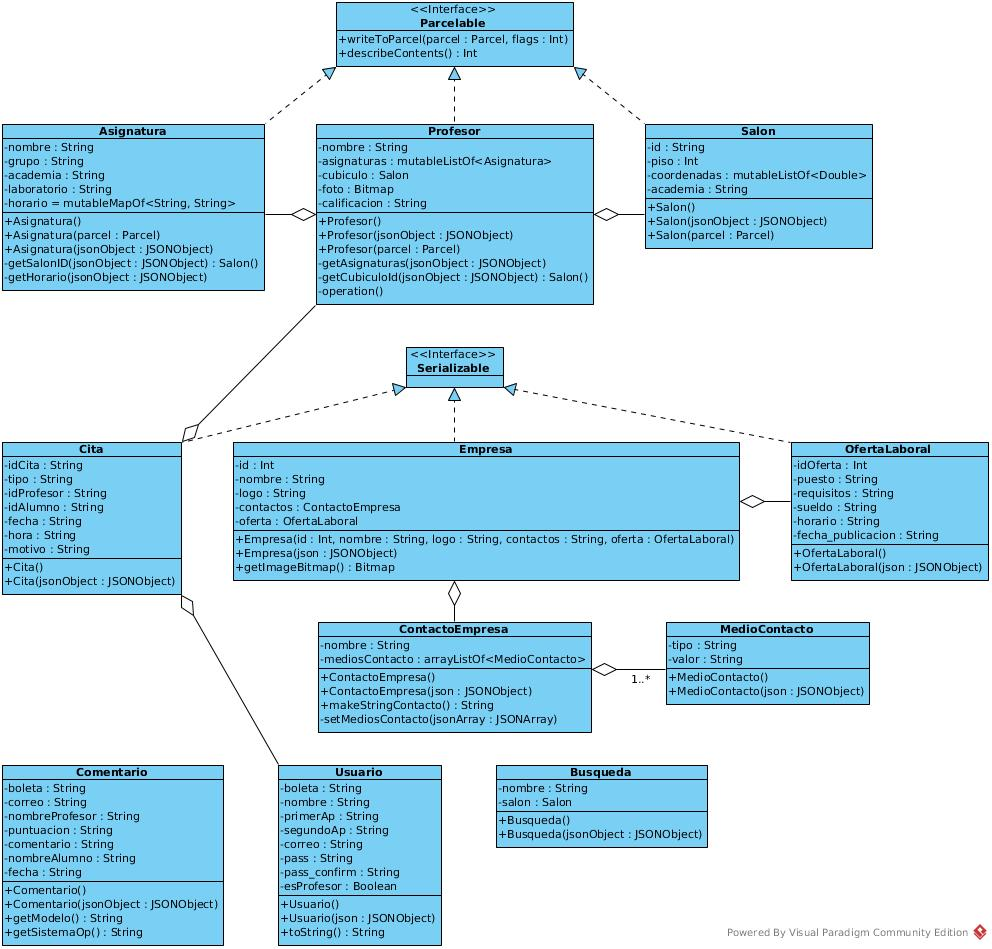
\includegraphics[width=1\textwidth]{images/clases/ModeloEntidad}
		\caption{Diagrama de clases: Modelo Entidad.}
		\label{fig:clasesModEntidad}
	\end{center}
\end{figure}

\begin{figure}[!htpb]
	\hypertarget{fig:clasesUtil}{\hspace{1pt}}
	\begin{center}
		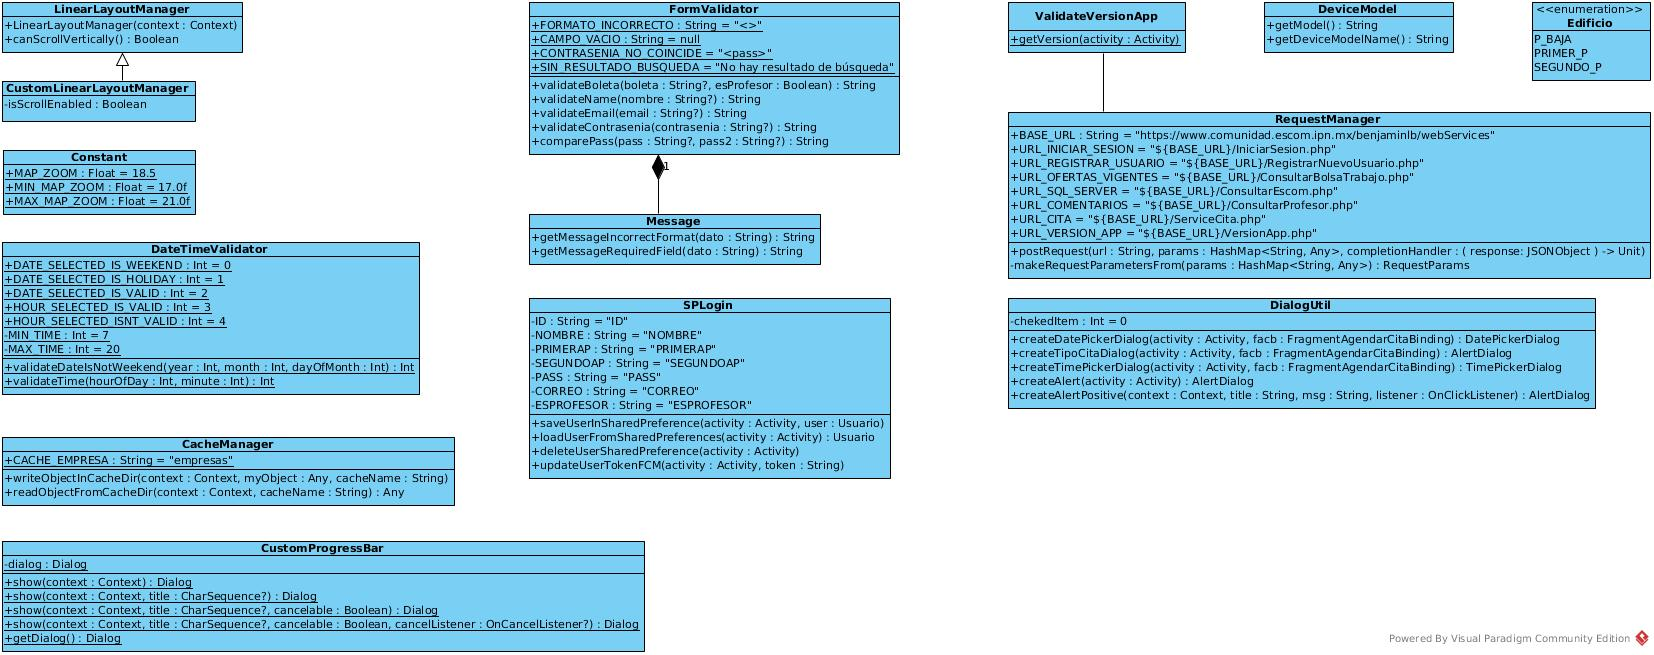
\includegraphics[width=1\textwidth]{images/clases/Util}
		\caption{Diagrama de clases: Util.}
		\label{fig:clasesUtil}
	\end{center}
\end{figure}

\begin{figure}[!htpb]
	\hypertarget{fig:clasesViewHolder}{\hspace{1pt}}
	\begin{center}
		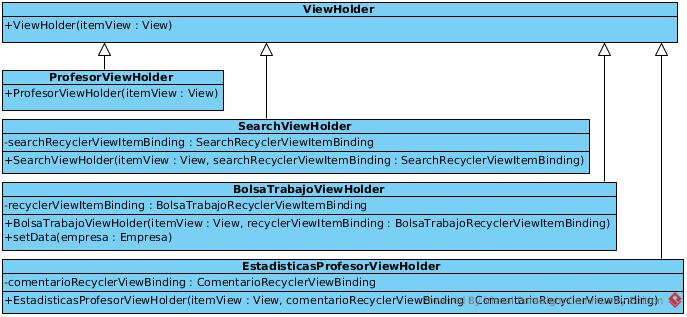
\includegraphics[width=1\textwidth]{images/clases/ViewHolder}
		\caption{Diagrama de clases: View Holder.}
		\label{fig:clasesViewHolder}
	\end{center}
\end{figure}

\begin{figure}[!htpb]
	\hypertarget{fig:clasesViewHolderAdapter}{\hspace{1pt}}
	\begin{center}
		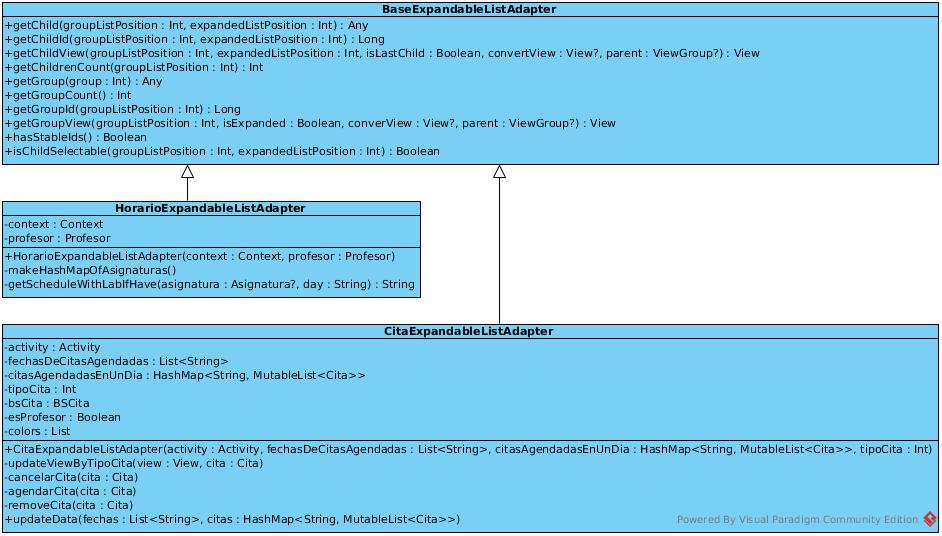
\includegraphics[width=1\textwidth]{images/clases/ViewHolderAdapterExpandable}
		\caption{Diagrama de clases: View Holder Adapter.}
		\label{fig:clasesViewHolderAdapter}
	\end{center}
\end{figure}

\begin{figure}[!htpb]
	\hypertarget{fig:clasesViewHolderTabAdapter}{\hspace{1pt}}
	\begin{center}
		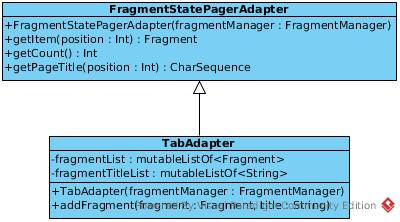
\includegraphics[width=1\textwidth]{images/clases/ViewHolderTabAdapter}
		\caption{Diagrama de clases: View Holder Tab Adapter.}
		\label{fig:clasesViewHolderTabAdapter}
	\end{center}
\end{figure}

\begin{figure}[!htpb]
	\hypertarget{fig:clasesViewModel}{\hspace{1pt}}
	\begin{center}
		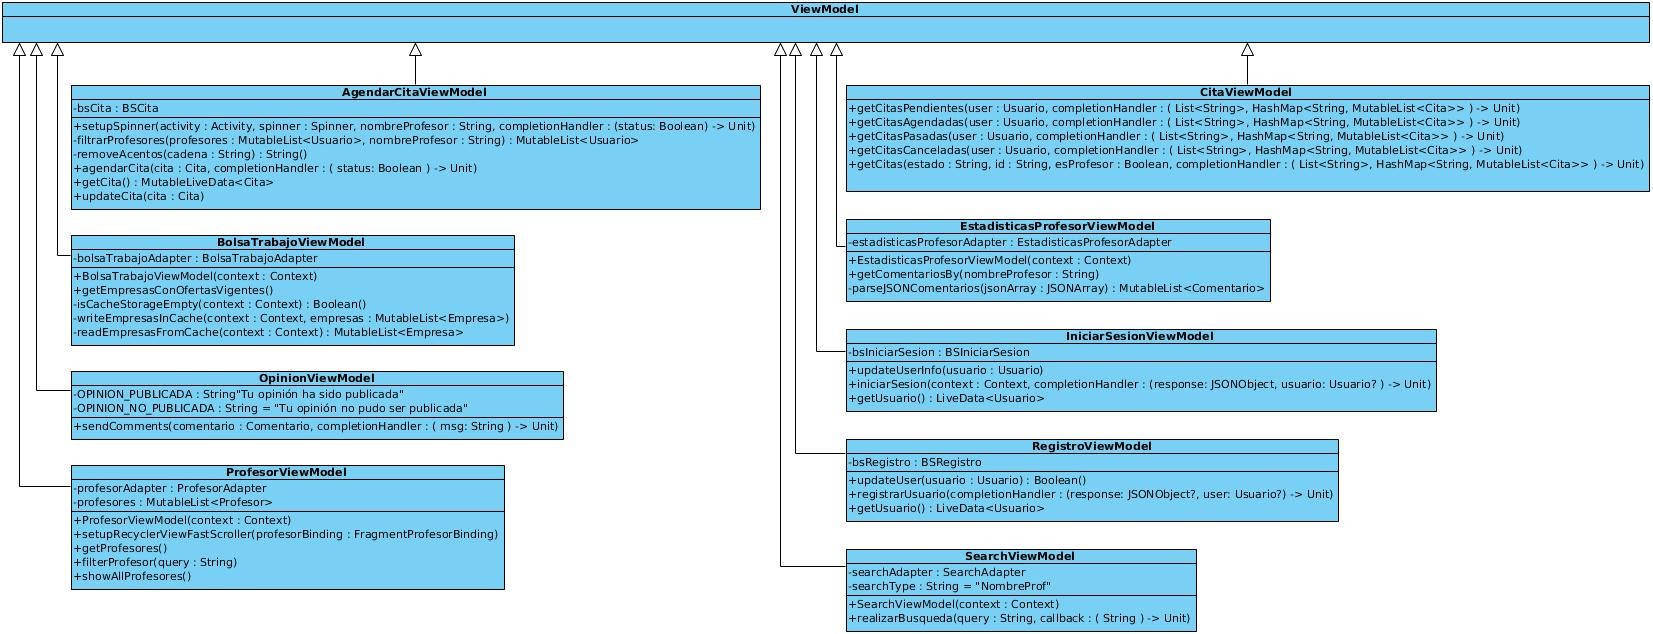
\includegraphics[width=1\textwidth]{images/clases/ViewModel}
		\caption{Diagrama de clases: View Model.}
		\label{fig:clasesViewModel}
	\end{center}
\end{figure}

\begin{figure}[!htpb]
	\hypertarget{fig:clasesVistaAct}{\hspace{1pt}}
	\begin{center}
		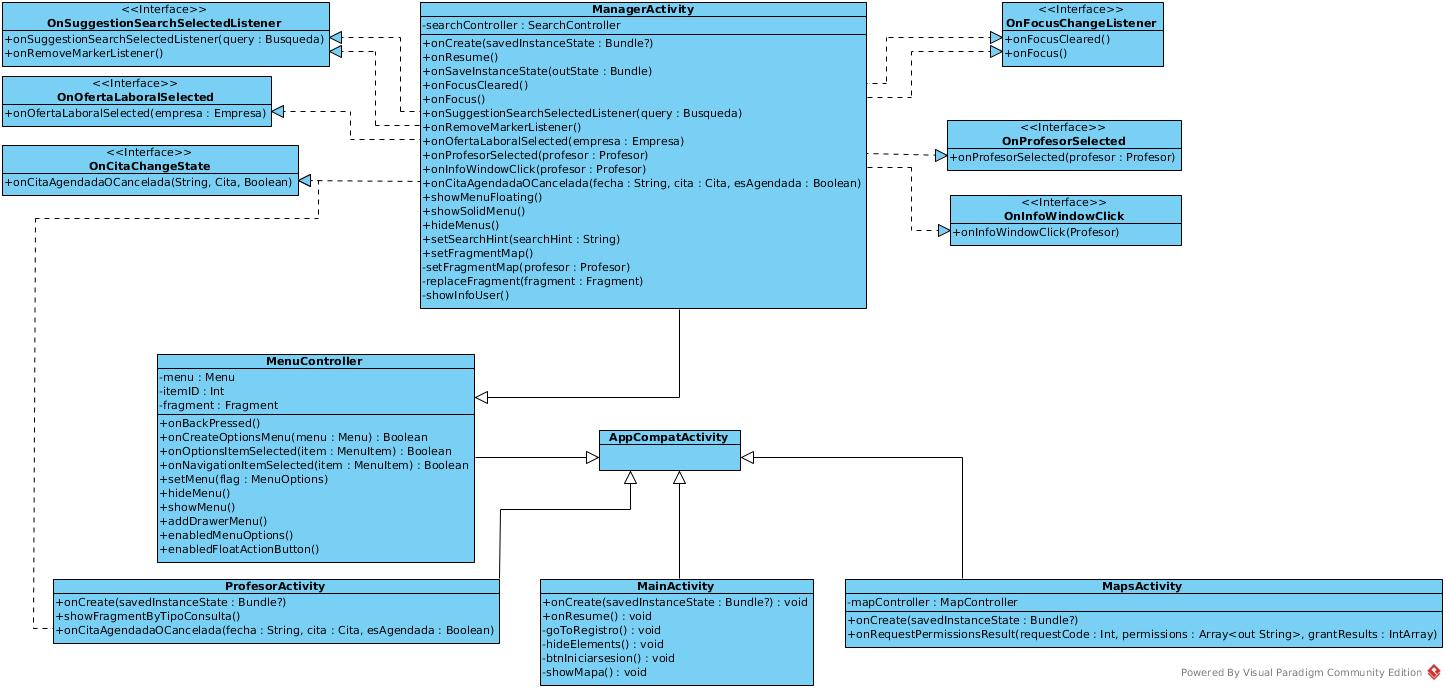
\includegraphics[width=1\textwidth]{images/clases/VistaActivity}
		\caption{Diagrama de clases: Vista Activity.}
		\label{fig:clasesVistaAct}
	\end{center}
\end{figure}

\begin{figure}[!htpb]
	\hypertarget{fig:clasesVistaFrag}{\hspace{1pt}}
	\begin{center}
		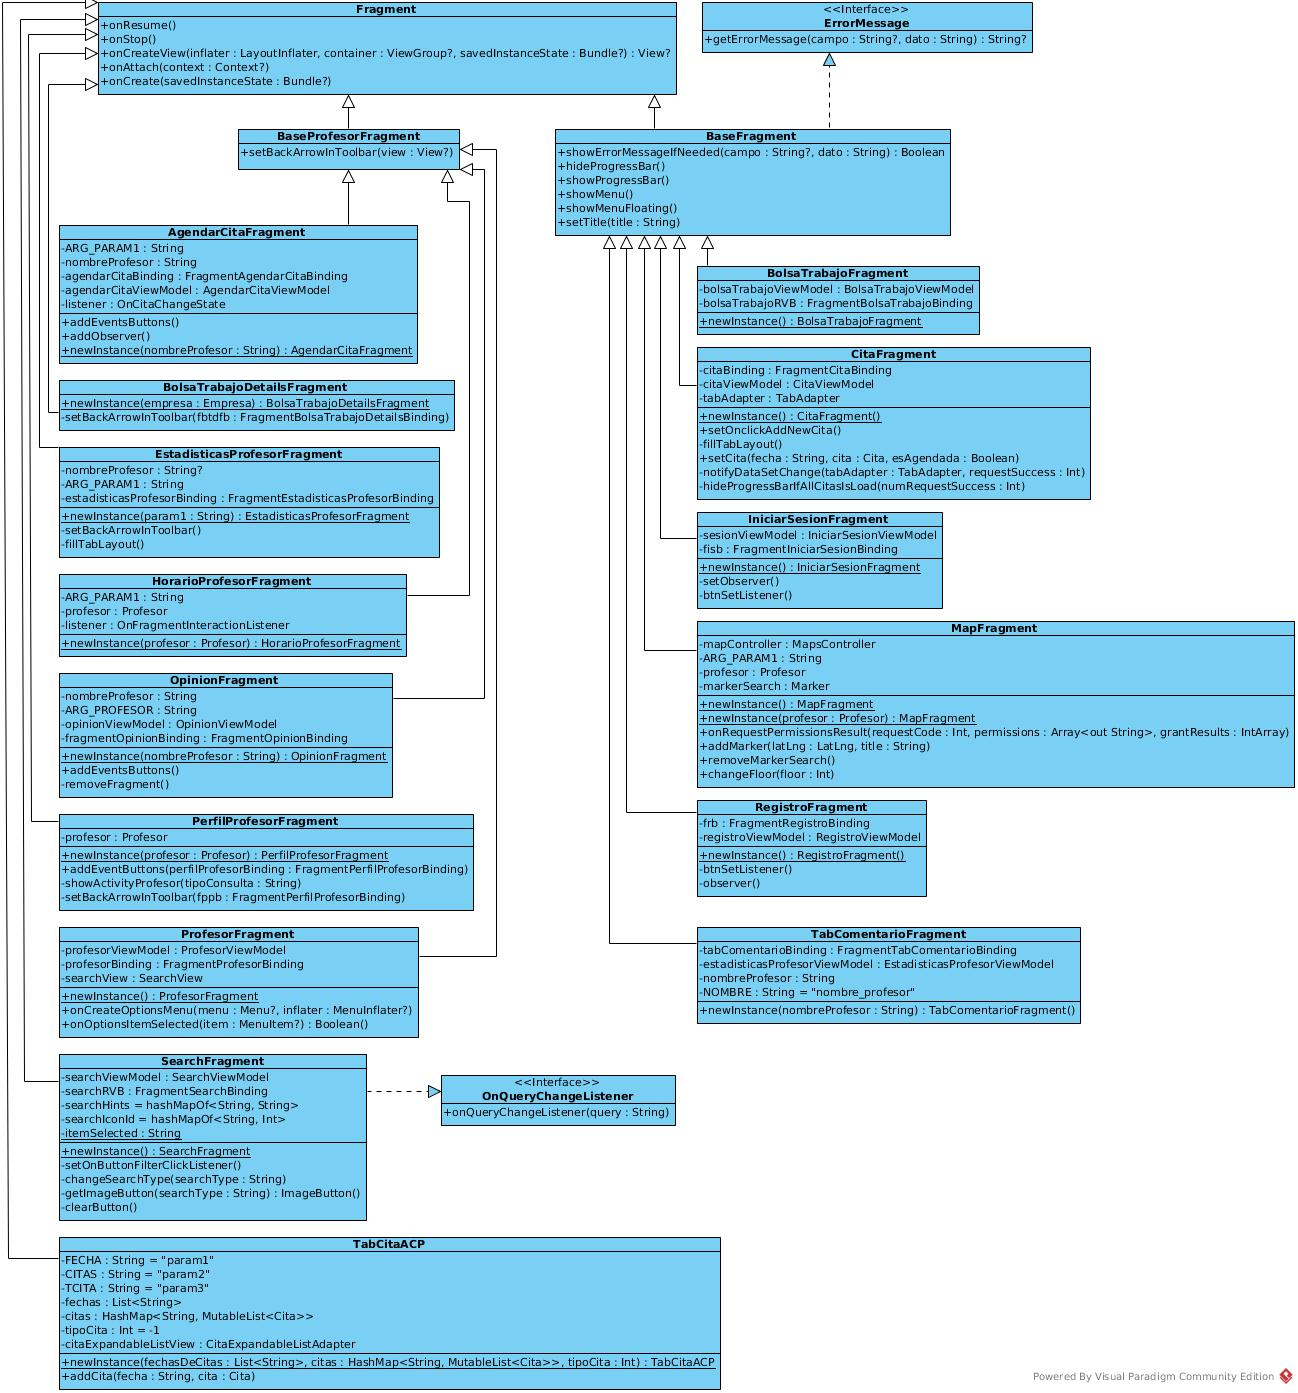
\includegraphics[width=1\textwidth]{images/clases/VistaFragment}
		\caption{Diagrama de clases: Vista Fragment.}
		\label{fig:clasesVistaFrag}
	\end{center}
\end{figure}

\newpage